\documentclass[unicode,11pt,a4paper,oneside,numbers=endperiod,openany]{scrartcl}
\usepackage{listings}
\usepackage{color}
\usepackage{graphicx}

\definecolor{dkgreen}{rgb}{0,0.6,0}
\definecolor{gray}{rgb}{0.5,0.5,0.5}
\definecolor{mauve}{rgb}{0.58,0,0.82}

\lstset{frame=tb,
  language=Java,
  aboveskip=3mm,
  belowskip=3mm,
  showstringspaces=false,
  columns=flexible,
  basicstyle={\small\ttfamily},
  numbers=none,
  numberstyle=\tiny\color{gray},
  keywordstyle=\color{blue},
  commentstyle=\color{dkgreen},
  stringstyle=\color{mauve},
  breaklines=true,
  breakatwhitespace=true,
  tabsize=3
}

\usepackage{ifthen}
\usepackage[utf8]{inputenc}
\usepackage{graphics}
\usepackage{graphicx}
\usepackage{hyperref}

\pagestyle{plain}
\voffset -5mm
\oddsidemargin  0mm
\evensidemargin -11mm
\marginparwidth 2cm
\marginparsep 0pt
\topmargin 0mm
\headheight 0pt
\headsep 0pt
\topskip 0pt        
\textheight 255mm
\textwidth 165mm

\newcommand{\duedate} {}
\newcommand{\setduedate}[1]{%
\renewcommand\duedate {Due date:~ #1}}
\newcommand\isassignment {false}
\newcommand{\setassignment}{\renewcommand\isassignment {true}}
\newcommand{\ifassignment}[1]{\ifthenelse{\boolean{\isassignment}}{#1}{}}
\newcommand{\ifnotassignment}[1]{\ifthenelse{\boolean{\isassignment}}{}{#1}}

\newcommand{\assignmentpolicy}{
\begin{table}[h]
\begin{center}
\scalebox{0.8} {%
\begin{tabular}{|p{0.02cm}p{16cm}|}
\hline
&\\
\multicolumn{2}{|c|}{\Large\textbf{HPC  2022 ---  Submission Instructions}}\\
\multicolumn{2}{|c|}{\large\textbf{(Please, notice that following instructions are mandatory: }}\\
\multicolumn{2}{|c|}{\large\textbf{submissions that don't comply with, won't be considered)}}\\
&\\
\textbullet & Assignments must be submitted to \href{https://www.icorsi.ch/course/view.php?id=14652}{iCorsi} (i.e. in electronic format).\\
\textbullet & Provide both executable package and sources (e.g. C/C++ files, Matlab). 
If you are using libraries, please add them in the file. Sources must be organized in directories called:\\
\multicolumn{2}{|c|}{\textit{Project\_number\_lastname\_firstname}}\\
& and  the  file must be called:\\
\multicolumn{2}{|c|}{\textit{project\_number\_lastname\_firstname.zip}}\\
\multicolumn{2}{|c|}{\textit{project\_number\_lastname\_firstname.pdf}}\\
\textbullet &  The TAs will grade your project by reviewing your project write-up, and looking at the implementation 
                 you attempted, and benchmarking your code's performance.\\

\textbullet & You are allowed to discuss all questions with anyone you like; however: (i) your submission must list anyone you discussed problems with and (ii) you must write up your submission independently.\\
\hline
\end{tabular}
}
\end{center}
\end{table}
}
\newcommand{\punkte}[1]{\hspace{1ex}\emph{\mdseries\hfill(#1~\ifcase#1{Points}\or{Points}\else{Points}\fi)}}


\newcommand\serieheader[6]{
\thispagestyle{empty}%
\begin{flushleft}

\includegraphics[width=0.4\textwidth]{usi_inf.png}
\end{flushleft}
  \noindent%
  {\large\ignorespaces{\textbf{#1}}\hspace{\fill}\ignorespaces{ \textbf{#2}}}\\ \\%
  {\large\ignorespaces #3 \hspace{\fill}\ignorespaces #4}\\
  \noindent%
  \bigskip
  \hrule\par\bigskip\noindent%
  \bigskip {\ignorespaces {\Large{\textbf{#5}}}
  \hspace{\fill}\ignorespaces \large \ifthenelse{\boolean{\isassignment}}{\duedate}{#6}}
  \hrule\par\bigskip\noindent%  \linebreak
 }

\makeatletter
\def\enumerateMod{\ifnum \@enumdepth >3 \@toodeep\else
      \advance\@enumdepth \@ne
      \edef\@enumctr{enum\romannumeral\the\@enumdepth}\list
      {\csname label\@enumctr\endcsname}{\usecounter
        {\@enumctr}%%%? the following differs from "enumerate"
	\topsep0pt%
	\partopsep0pt%
	\itemsep0pt%
	\def\makelabel##1{\hss\llap{##1}}}\fi}
\let\endenumerateMod =\endlist
\makeatother




\usepackage{textcomp}





\begin{document}

\setassignment
\setduedate{12.10.2022 (midnight)}

\serieheader{High-Performance Computing Lab}{2022}{Student: SIMONE TARENZI}{Discussed with: E. BARDELLI, L. ZANIOL, V. NAIK}{Solution for Project 1}{}
\newline

\section{Explaining Memory Hierarchies \punkte{25}}
1. From the graph obtained by running the program on the compute node of the cluster, there seems to be pretty clear "steps" where the time to read and write data quickly rises. 
\begin{center}
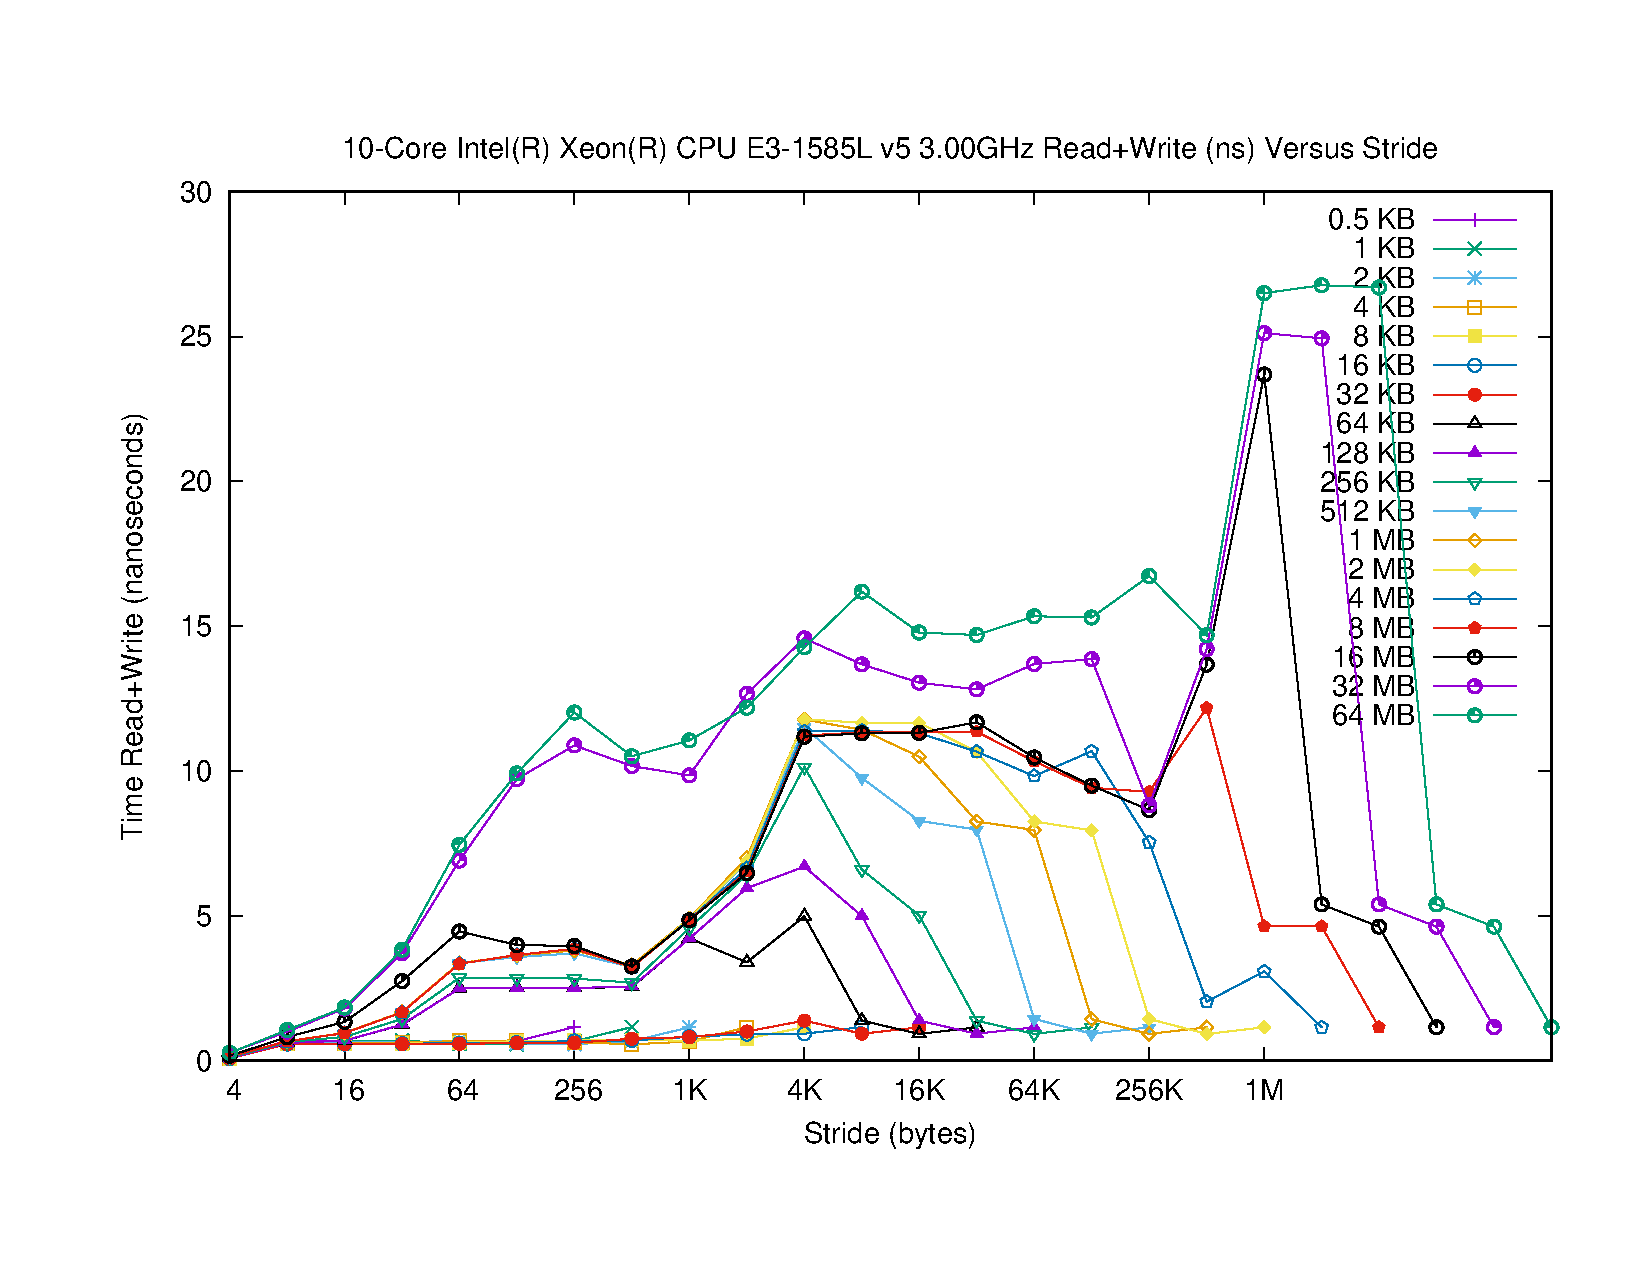
\includegraphics[width=0.7\linewidth]{gnuplot_ics_cluster.pdf}
\end{center}
Looking at the various lines, it seems that the 64 KB one is the first which starts to deviate from the previous ones, so my guess is that 32 KB is the size of the L1 cache of the compute node processor.
\newline
After that, results are a bit harder to interpret: from the 64 KB to the 4 MB line, they all follow pretty much the same trajectory. My guess would have been 128 KB for the L2 cache size and 8 MB for L3 cache, but that wasn't actually the case.
\newline
Using the command "likwid-topology" we can take a look at the actual sizes:
\begin{center}
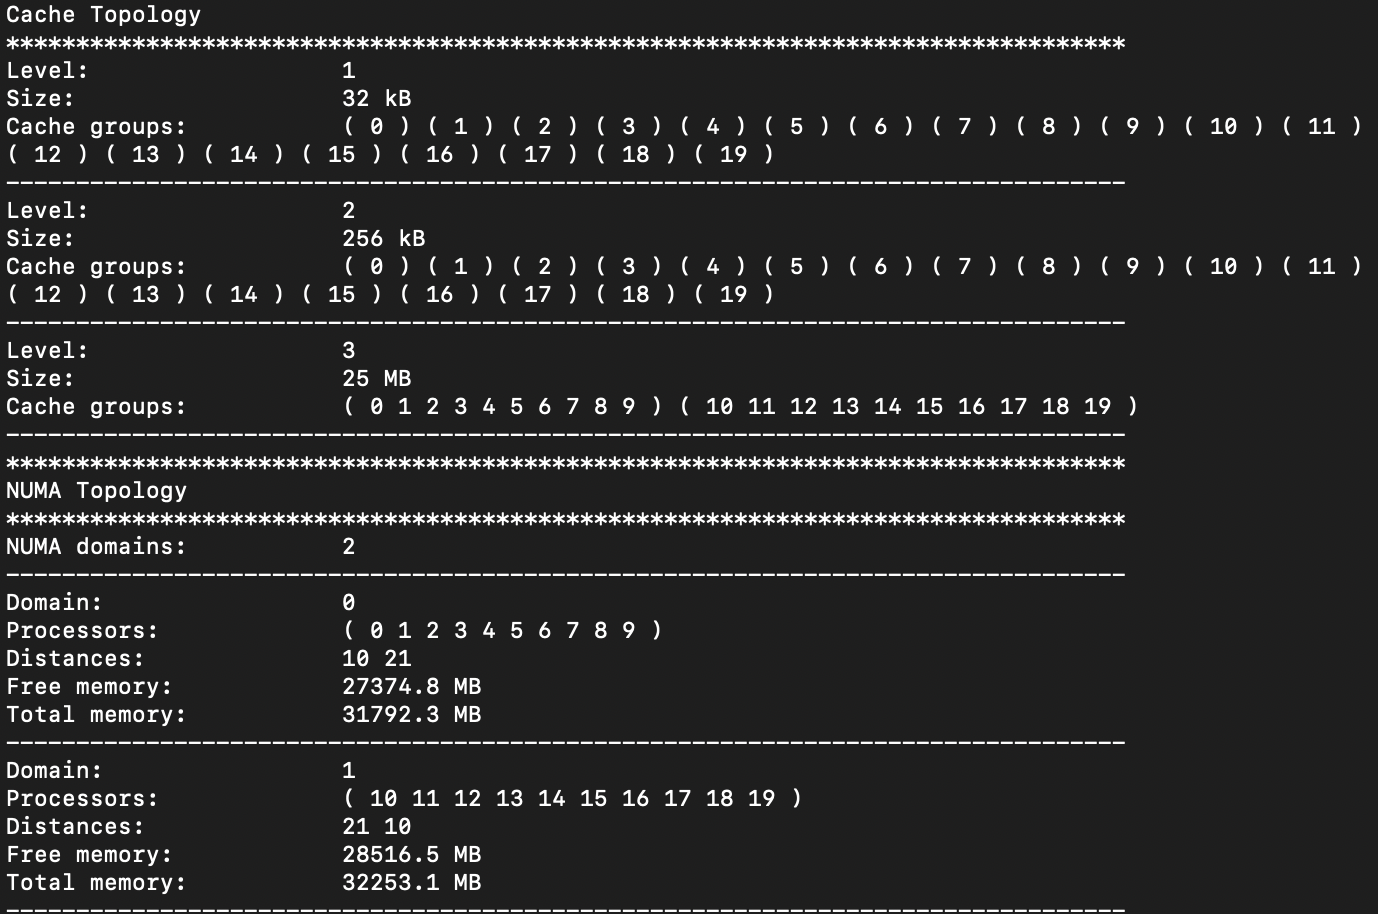
\includegraphics[width=0.6\linewidth]{cache_topology.png}
\end{center}
L1 cache: 32 KB
\newline
L2 cache: 256 KB
\newline
L3 cache: 25 MB
\newline
Main Memory: 64 GB
\newline
\newline
3. In both cases at csize = 128 KB with stride = 8 KB and at csize = 1 MB  with stride = 512 KB we are accessing the L1 cache in linear time.
\newline
\newline
4. We will have good temporal locality when we are accessing data which is stored in the same cache layer: for example all array sizes up until 32 KB share the same temporal locality, since they can be stored in L1 cache. Array sizes such as 32 and 64 MB instead only show ok temporal locality from 4 to 256 KB stride, because they are so big that they will have trouble getting accessed in the same cache layer.
\newline
Array sizes from 512 KB to 8 MB show instead two clear plateaus where I'm guessing they switch from L2 to L3 cache layer.
\newline
\newline
Finally let's take a look at the performance graph of an M1 Pro Macbook Pro.
\begin{center}
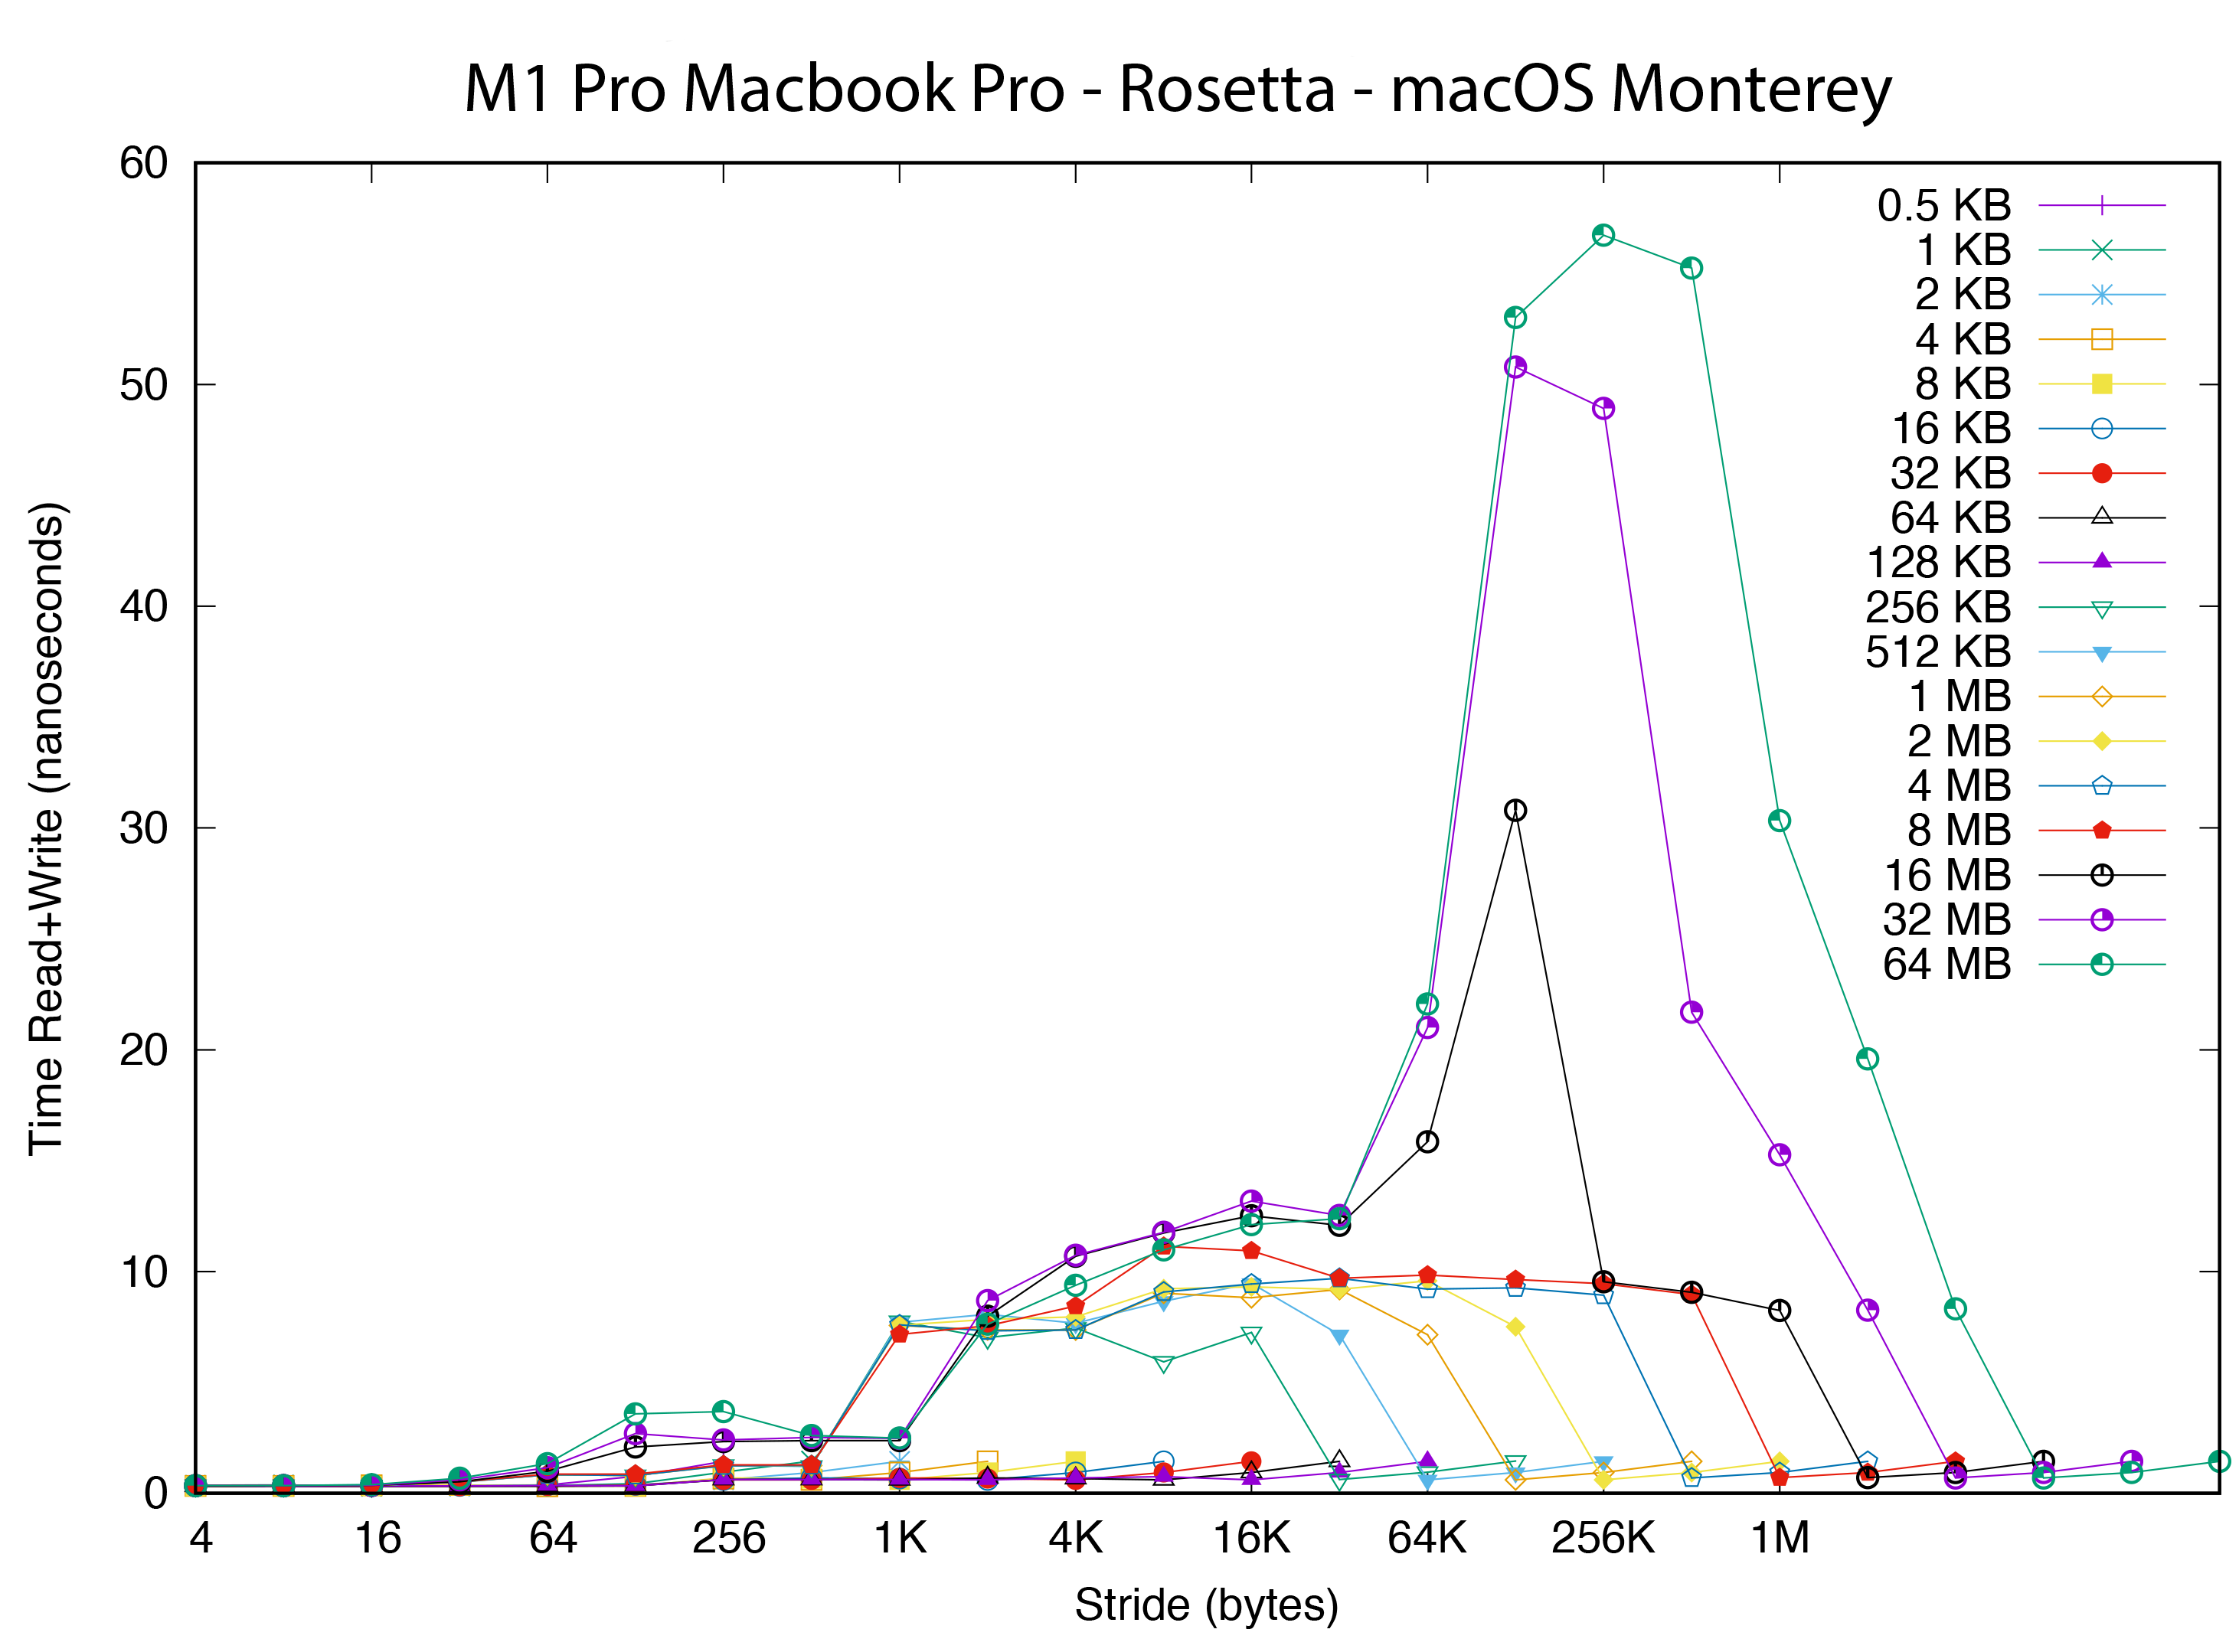
\includegraphics[width=0.7\linewidth]{gnuplot_local_machine.png}
\end{center}
Having 2.9 MB of L1, 28 MB of L2 and 24 MB of L3 cache helps getting good temporal locality at array sizes up to 16 MB at all stride values.

\section{Optimize Square Matrix-Matrix Multiplication  \punkte{60}}
The optimization had the objective of implementing a way to multiply matrices using submatrices of NxN cells at a time: this enables saving more of those numbers in localized, faster to access memory, and then, after the calculations are done, saving them back into the resulting matrix.  This would result in less accesses to the slow memory where the matrices are stored and, therefore, improve performance.
\newline
The idea was to implement a way to do that for all matrices, no matter their dimensions: all calculations would be done in blocks of 2x2 and then, once close to the boundaries of the matrix, go back to the previous naive implementation. Sadly I wasn't able to do that, so instead I've implemented a way to check if the matrix dimensions are divisible by 2 or 3, and then use blocks of 2 or 3, respectively.
\newline
This, however, gives no speed benefit to calculations done on matrices whose dimensions aren't divisible by 2 or 3, like all prime numbers for example, but since the program is multiplying matrices of various sizes, there will still be an overall increase in speed.
\begin{lstlisting}
void square_dgemm (int n, double* A, double* B, double* C){
	int i,j,k;
	if (the matrix is divisible in blocks of 3x3){
		for (i=0; i<n3; i+=3){
			for (j=0; j<n3; j+=3){
				//save each cell of this block in local variables
				double c0 = C(i,j);
				double c1 = C(i,j+1);
				double c2 = C(i,j+2);
				double c3 = C(i+1,j);
				//etc until c8
				for (k = 0; k < n; k++){
					//save the results in the local variables
					c0 += A(i,k) * B(k,j);
					c1 += A(i,k) * B(k,j+1);
					c2 += A(i,k) * B(k,j+2);
					c3 += A(i+1,k) * B(k,j);
					//etc
				}
				//save the final calculations back in to the matrix
				C(i,j) = c0;
				C(i,j+1) = c1;
				C(i,j+2) = c2;
				C(i+1,j) = c3;
				//etc
			}
		}
	}
	else if (the matrix is divisible in blocks of 2x2){
		//same thing but there will be 4 local variables
	}
	else if (the matrix is not divisible by 3 or 2){
		//use the naive implementation
	}
}
\end{lstlisting}
Some matrices will obviously be divisible by both 2 and 3, this is why the code checks with 3 first, so that in those cases it can always use the faster implementation.
\newline
\newline
First of all, let's take a look at the performance of the implementation of 2x2 blocks alone.
\begin{center}
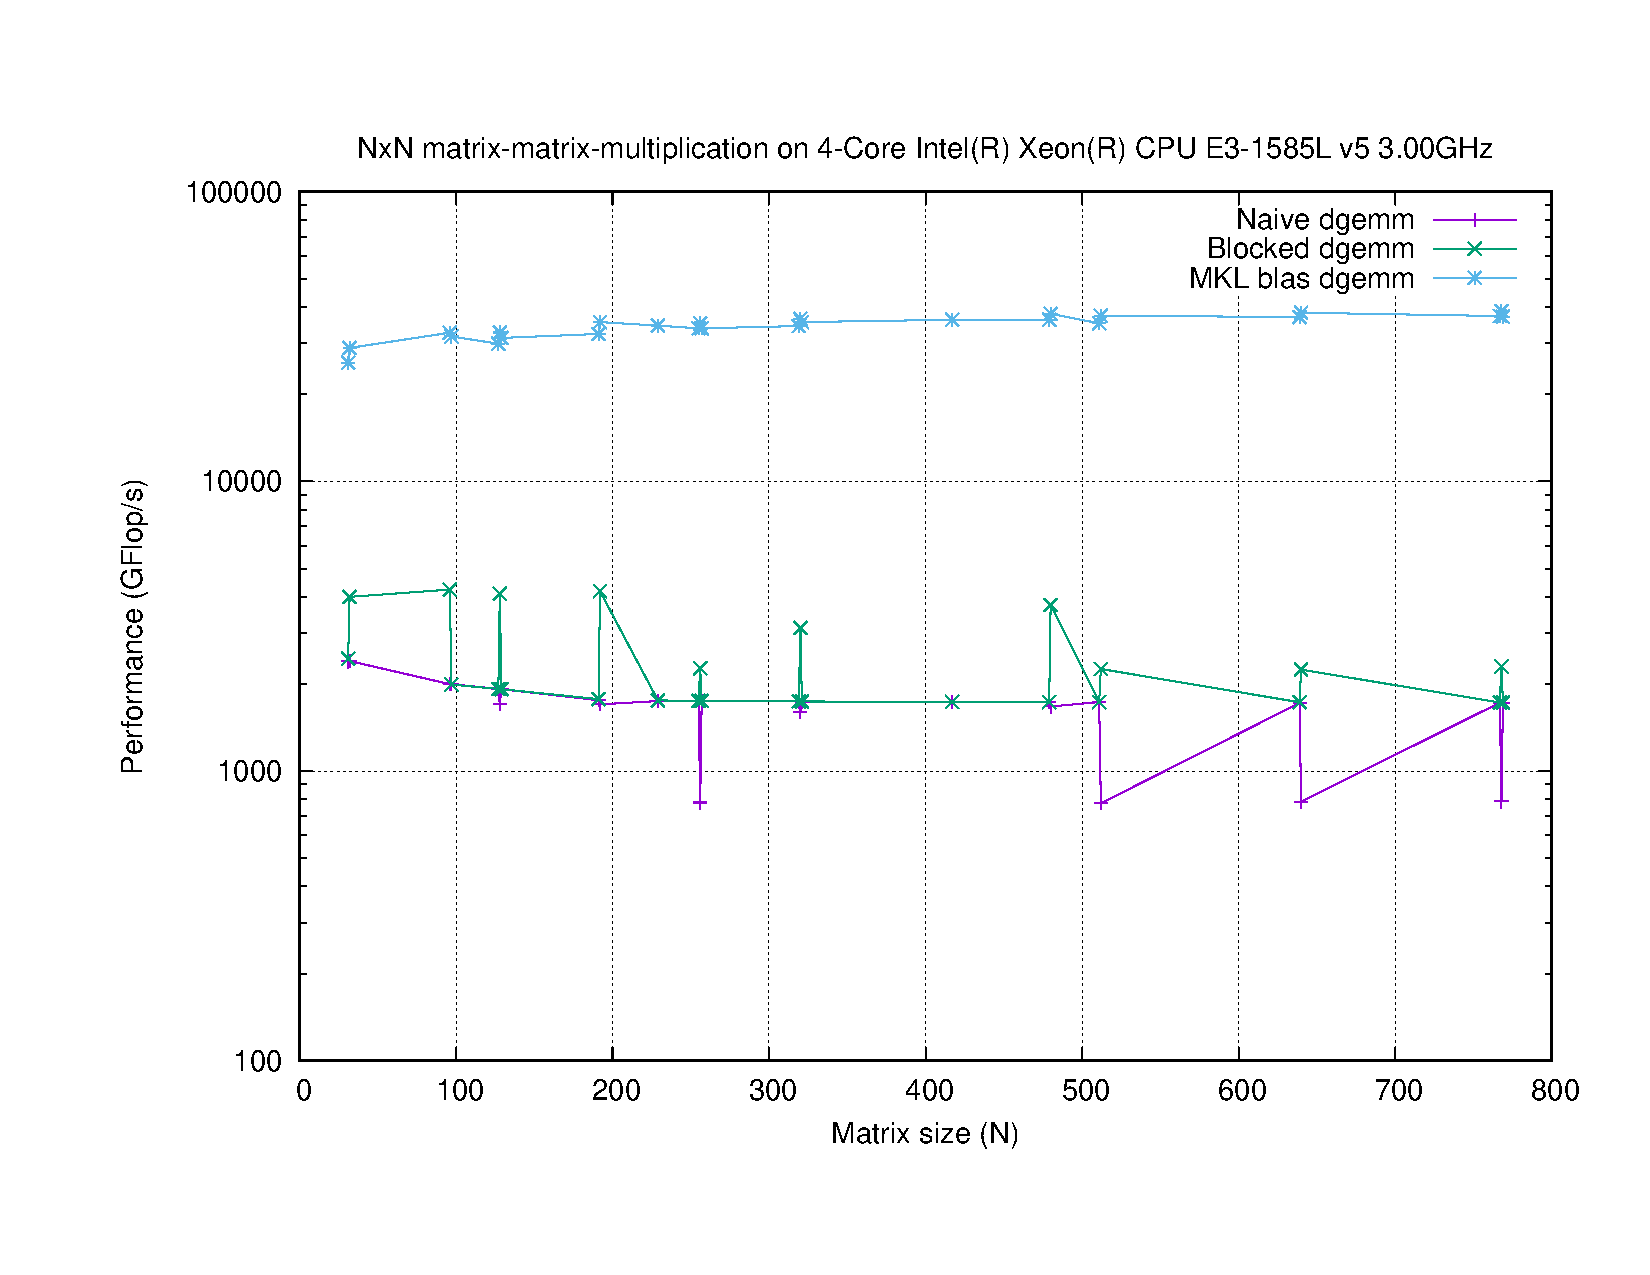
\includegraphics[width=0.7\linewidth]{timing_2x2_blocks_only_even_matrices.pdf}
\end{center}
Only even matrices get an improvement in performance, but those that do are 2 to 2.5 times as fast as the ones that use the naive implementation. For example, for matrix size 128, the peak speed went from 1713.7 Mflop/s to 4218.25 Mflop/s.
\newline
\newline
Now let's look at the final implementation with both 3x3 and 2x2 blocks.
\begin{center}
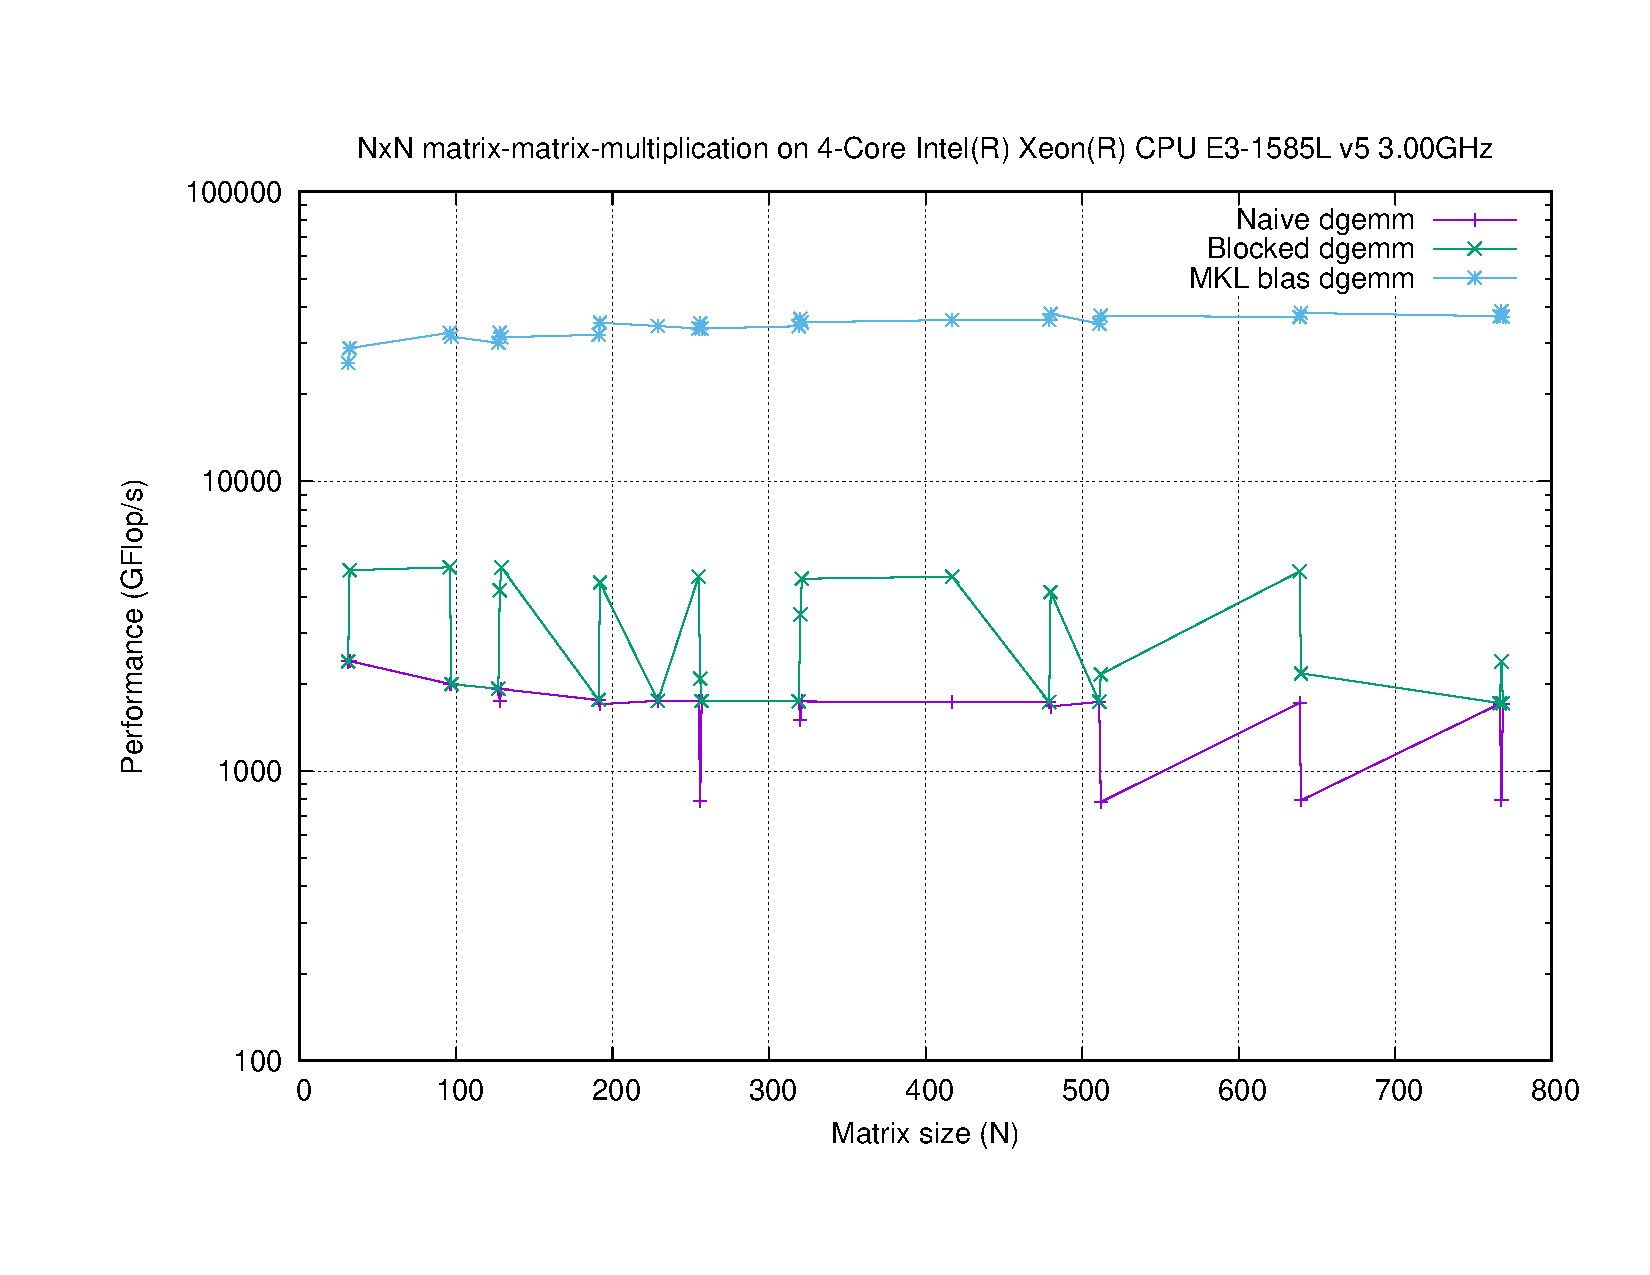
\includegraphics[width=0.7\linewidth]{timing_3x3_and_2x2.pdf}
\end{center}
More matrices now get an improvement in performance, and the ones divisible by blocks of 3x3 now get 2.5 times the performance of the naive implementation as a basis: matrix size 129 went from 1919.15 Mflop/s to 5056.54 Mflop/s.
\newline
In the end the performance of the whole program went from a 4.5 peak percentage to an 8 percent peak.
\newline
\newline
I was actually thinking of adding an implementation that used 4x4 blocks too but, surprisingly, it performed slightly worse than the implementation with both 2x2 and 3x3 blocks.
\begin{center}
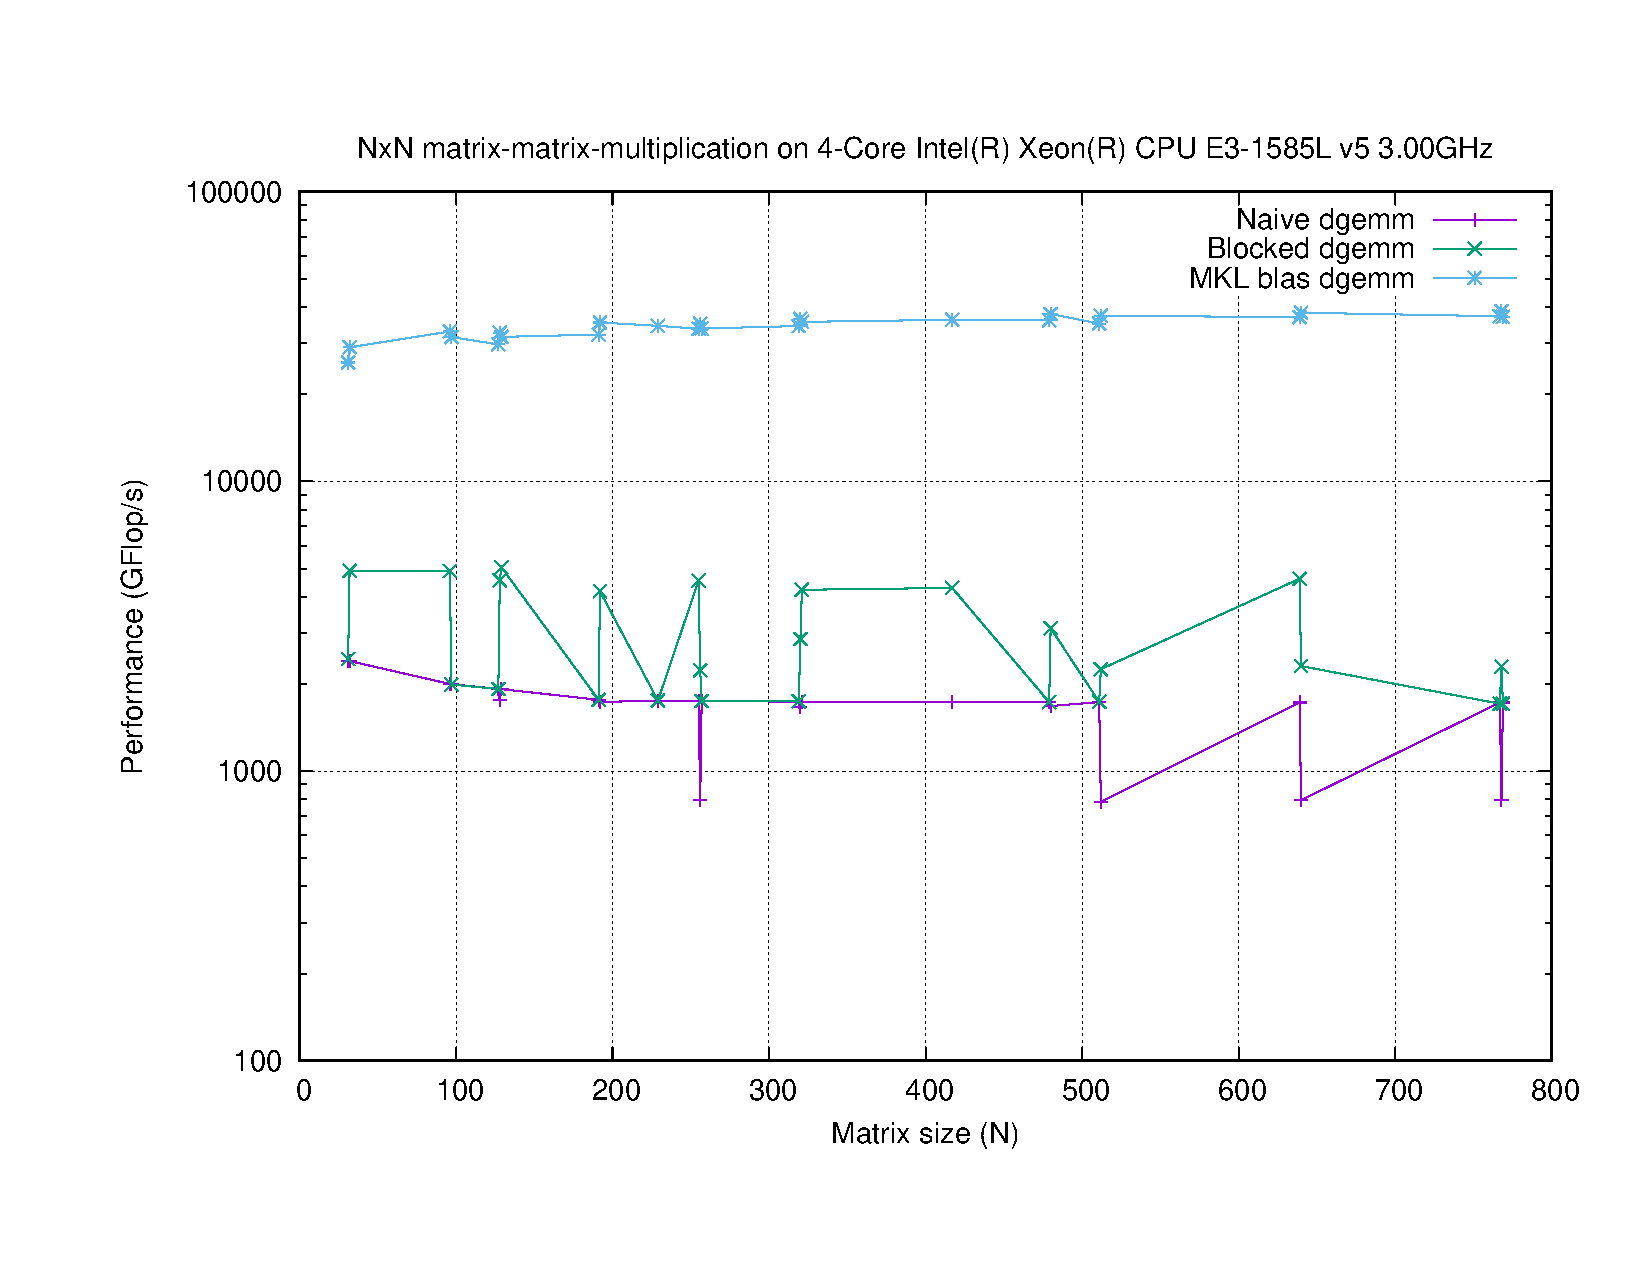
\includegraphics[width=0.7\linewidth]{timing_4x4_3x3_2x2.pdf}
\end{center}
To see the actual impact that local variables can have, I tried to see what would happen after removing the one in the naive implementation.
\begin{center}
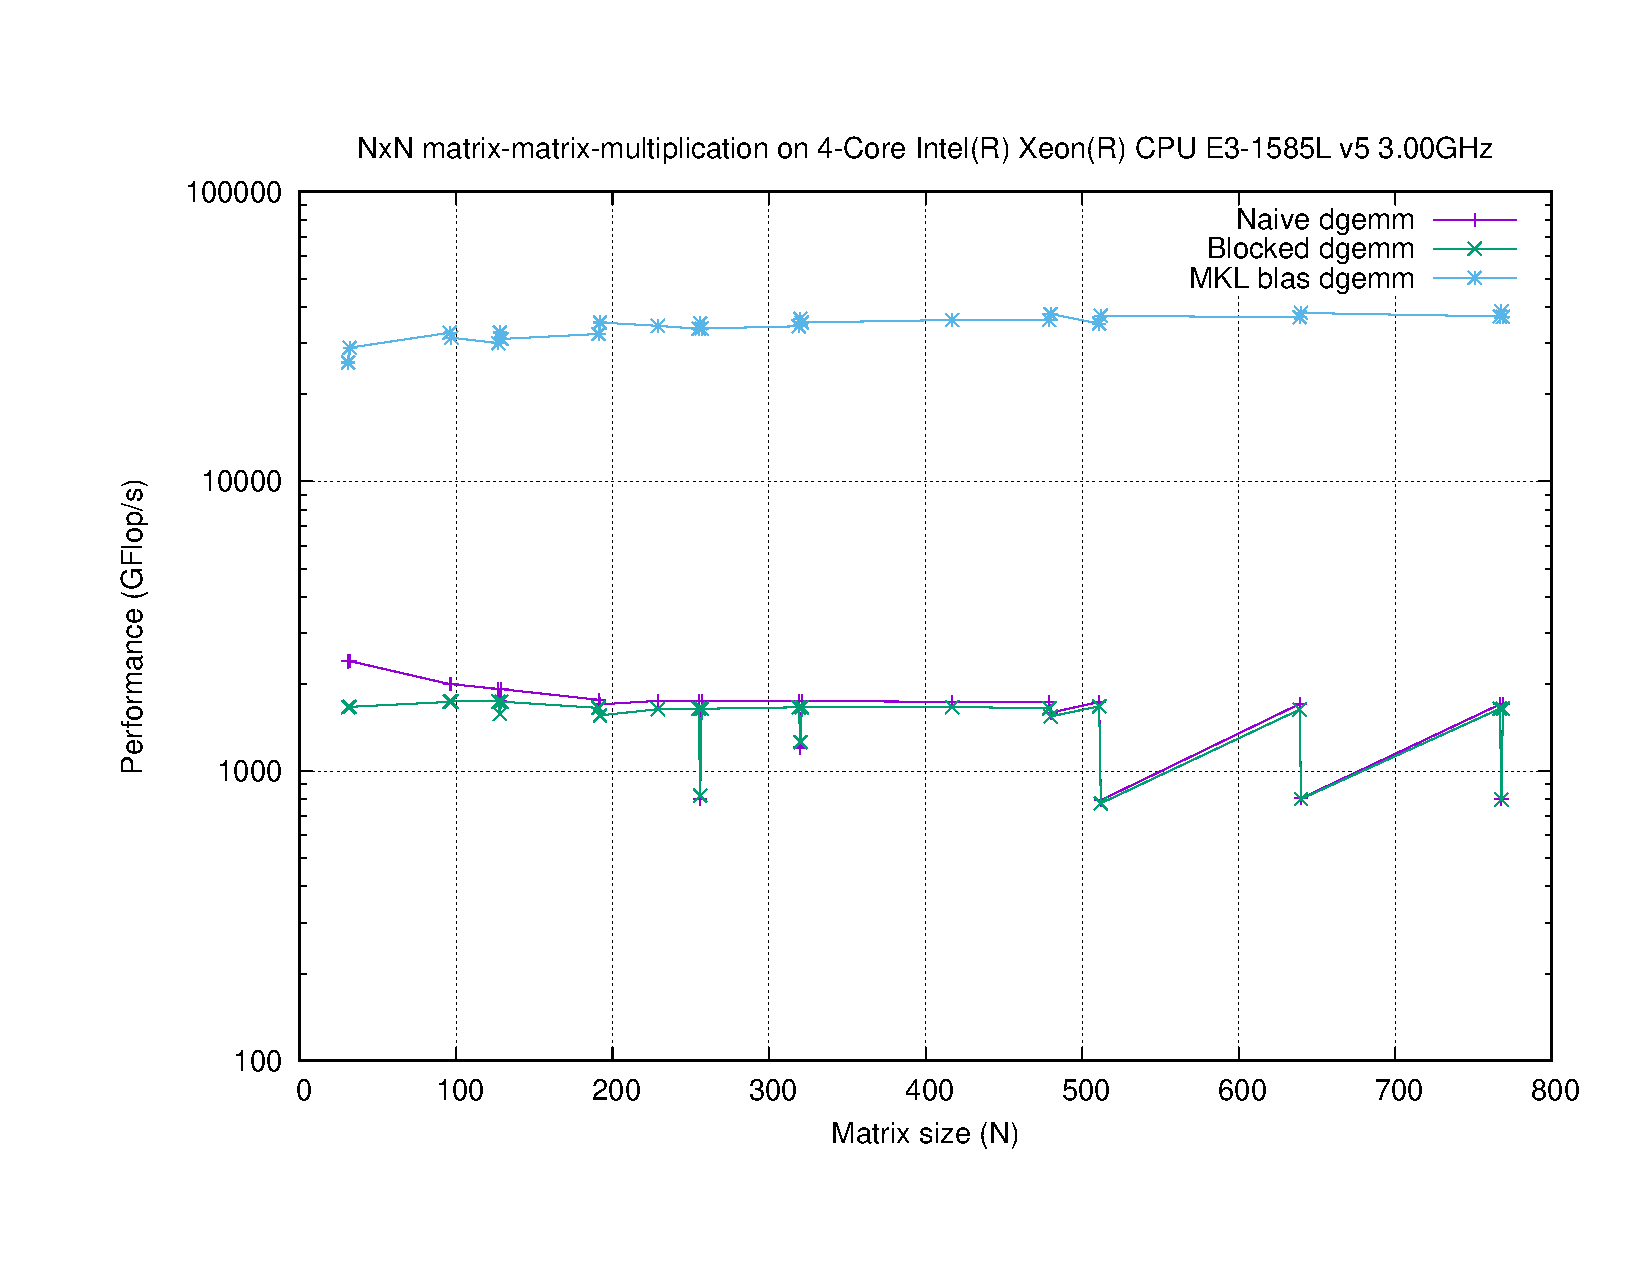
\includegraphics[width=0.7\linewidth]{timing_removed_local_sum.pdf}
\end{center}
It's not much when it's just a single one, but we've already seen how much of a difference they can make when there's multiple accesses to the same ones over and over again.
\newline
\newline
And, finally, one last test where the order of the j and k indeces gets flipped.
\begin{center}
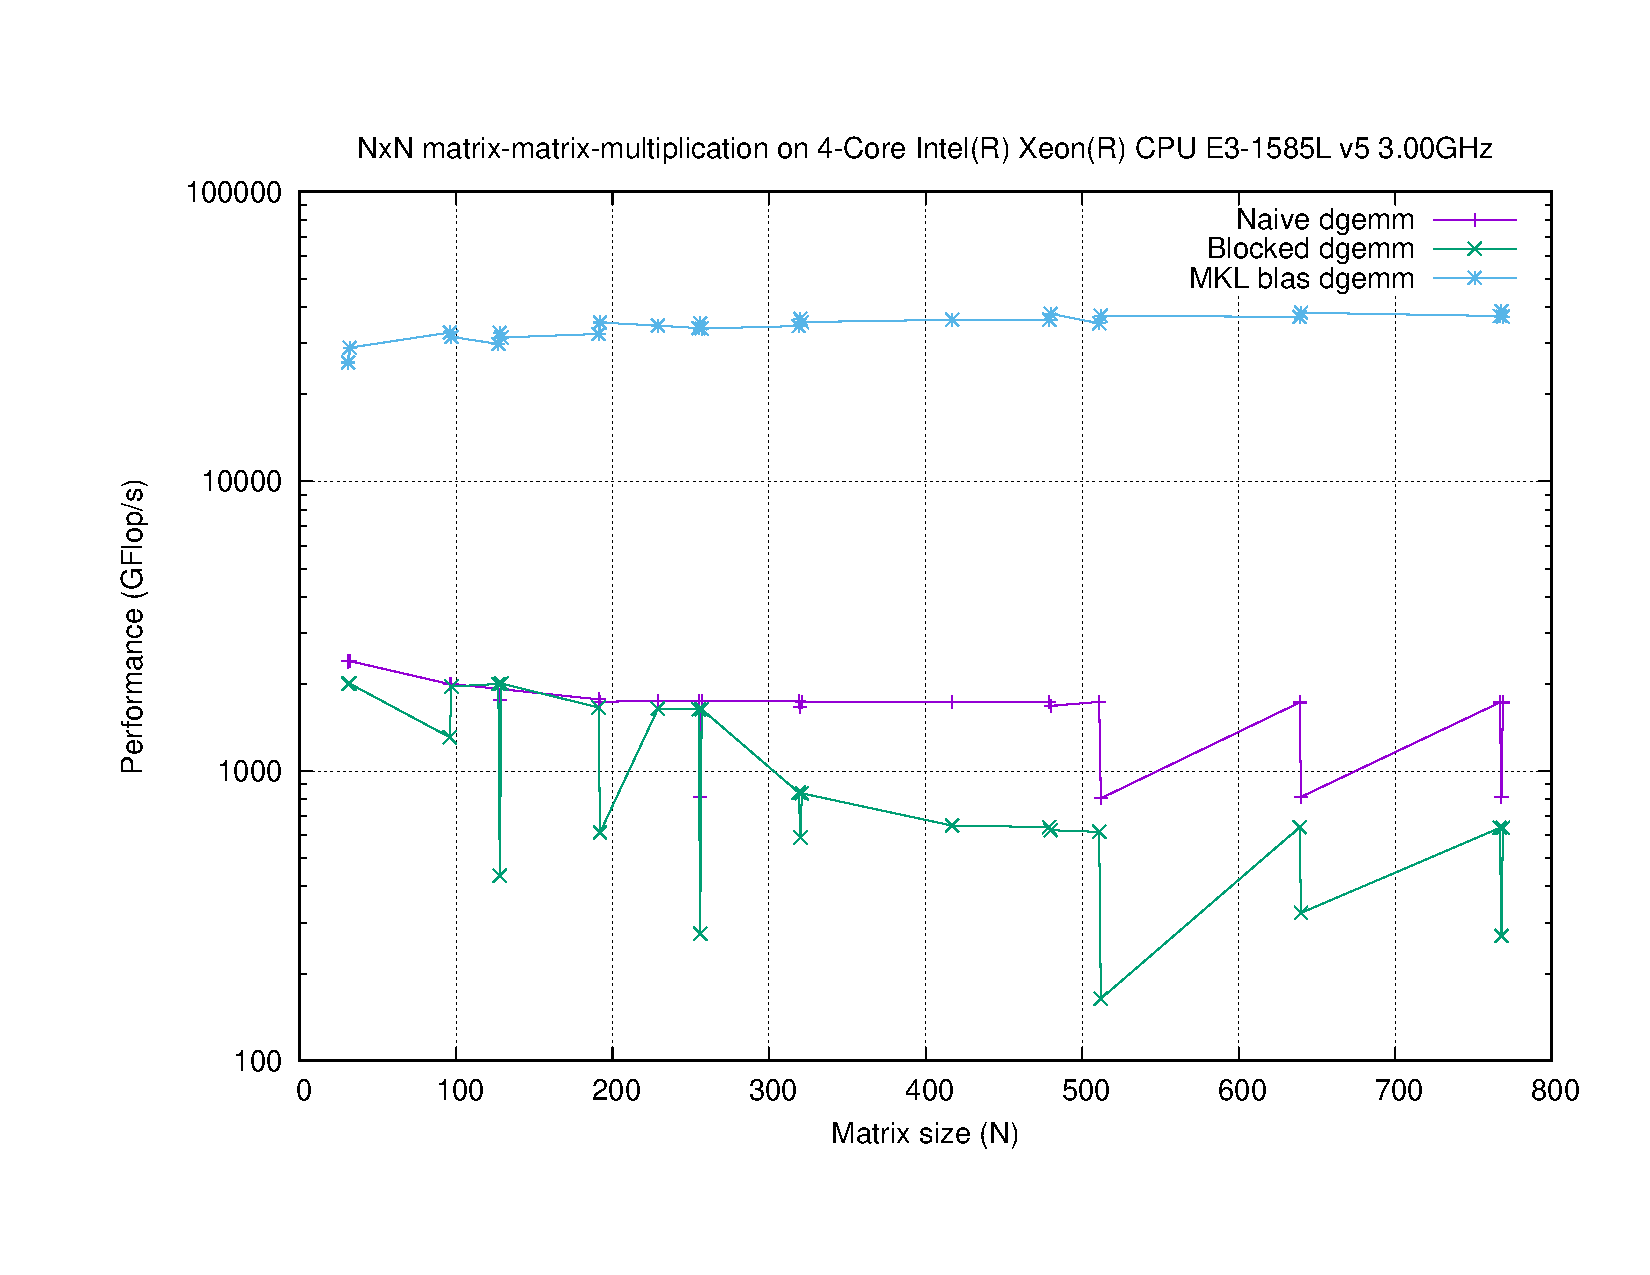
\includegraphics[width=0.7\linewidth]{timing_reverse_k_j_index.pdf}
\end{center}

\section{Quality of the Report  \punkte{15}}


\end{document}
